\chapter{Metodología}

Para el correcto desarrollo de este Trabajo Fin de Grado se ha establecido una metodología estructurada en cuatro fases incrementales, combinando la investigación teórica, la validación conceptual y el diseño artístico con el desarrollo iterativo de software. Este enfoque escalonado permite abordar las limitaciones de tiempo y recursos propias de un proyecto académico individual, asegurando que la arquitectura base sea sólida antes de proceder a la construcción del prototipo jugable.

\section{Fases de Desarrollo del Proyecto}
El flujo de trabajo proyectado abarca desde la conceptualización inicial hasta la validación de la demo funcional. En la Figura~\ref{fig:fases-metodologia} se muestra el esquema general de las etapas que articulan la metodología del proyecto.

\begin{figure}[H]
  \centering
  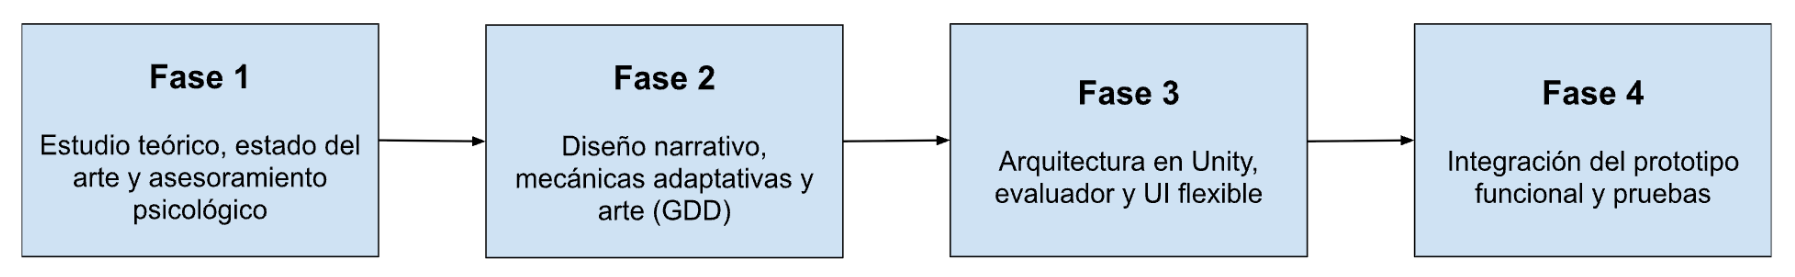
\includegraphics[width=0.8\textwidth]{fases.png}
  \caption{Diagrama de las fases incrementales de la metodología del proyecto}
  \label{fig:fases-metodologia}
  \fuente{elaboración propia}
\end{figure}

A continuación, se detalla el alcance y las tareas específicas que comprenden cada una de las cuatro etapas metodológicas:
\begin{enumerate}
  \item \textbf{Fase 1. Estudio teórico, documentación y asesoramiento psicológico:} el primer paso metodológico ha consistido en la revisión bibliográfica sobre narrativa digital \parencite{navarro2023}, narrativa ambiental \parencite{finestrat2018, boyero2025}, consonancia ludonarrativa \parencite{hernandez2024} y construcción de la identidad a través de la agencia \parencite{cuadrado2020, gomez2026}. Paralelamente, se han analizado obras de referencia que destacan bien por su tratamiento de la salud mental y la identidad como \textit{Celeste} \parencite{maddy2018}, \textit{Gris} \parencite{nomada2018}, \textit{Night in the Woods} \parencite{infinitefall2017} o \textit{Tell Me Why} \parencite{dontnod2020}, o bien por la utilización de sistemas de perfilado psicológico y adaptación al jugador como \textit{Silent Hill: Shattered Memories} \parencite{climax2009}, \textit{Undertale} \parencite{fox2015} o \textit{Disco Elysium} \parencite{zaum2020}. Asimismo, dado el compromiso del proyecto con la representación respetuosa de la perspectiva de género y la salud mental, esta fase incorpora sesiones de consulta y asesoramiento con una especialista en psicología con el fin de validar que la representación de la crisis identitaria y las estrategias de afrontamiento carezcan de estigmas o estereotipos dañinos. Para todas las referencias se ha adoptado la normativa estándar de citación APA conforme al Libro de Estilo de la \ac{EPS} \parencite{eps2015}.
  \item \textbf{Fase 2. Diseño narrativo, artístico y de mecánicas (\ac{GDD}):} a partir de las conclusiones extraídas en la investigación previa, se elabora el Documento de Diseño de Juego. En esta etapa se estructura el arco narrativo introspectivo dividido en tres mundos abstractos y las condiciones que modulan su desenlace abierto. En el plano mecánico, se definen los eventos concretos que alimentan el evaluador en segundo plano, las reglas de los mecanismos y la matriz de transformación de habilidades e interfaz. En el apartado visual, se establece la dirección artística en \ac{2D} con profundidad 2.5D bajo perspectiva cenital oblicua (\textit{top-down} 3/4), definiendo las paletas cromáticas evolutivas, el diseño de \textit{sprites} del avatar y de las manifestaciones abstractas, la iluminación ambiental y la maquetación de la interfaz adaptativa.
  \item \textbf{Fase 3. Desarrollo técnico de la arquitectura base en Unity:} antes de construir los niveles definitivos, el trabajo técnico se centra en programar los cimientos modulares del sistema en C\#. En primer lugar, se diseña una arquitectura desacoplada basada en eventos y contenedores de datos (\textit{ScriptableObjects}) capaz de modificar parámetros del jugador y del lienzo (\textit{Canvas}) en tiempo real sin comprometer la estabilidad de la ejecución. En segundo lugar, se implementa el módulo observador en segundo plano encargado de contabilizar las métricas de interacción del usuario y calcular los pesos conductuales que disparan las propuestas de adaptación.
  \item \textbf{Fase 4. Construcción iterativa del prototipo funcional y pruebas:} la última etapa aborda la construcción de un prototipo funcional jugable (demo o \textit{vertical slice}) que permita experimentar en la práctica la transición entre los estados del juego. Se integran las escenas en Unity, ordenación en el eje vertical (\textit{Y-Sorting}) e iluminación \ac{URP} \ac{2D}, procediendo finalmente a la realización de pruebas funcionales para verificar que la recolección de eventos, el panel de consentimiento y el cambio de habilidades funcionen de manera fluida.
\end{enumerate}

\section{Herramientas y Justificación Tecnológica}
Para llevar a cabo las distintas fases del proyecto se ha seleccionado el siguiente conjunto de herramientas de software:

\subsection{Motor Gráfico: Justificación de Unity}
El motor principal elegido para el desarrollo del videojuego es Unity \parencite{unity2023}. Su elección frente a otras alternativas del mercado responde a criterios técnicos alineados con los requisitos de este TFG:
\begin{itemize}
    \item Especializado en 2D: Unity cuenta con un conjunto de herramientas 2D maduras (\textit{Sprite Editor}, \textit{Tilemap}, \textit{2D Lighting}, animación por \textit{sprites}\ldots) \parencite{unity2023}, ideal para materializar la dirección artística de los mundos abstractos y las transiciones atmosféricas.
    \item Arquitectura basada en componentes y C\#: permite diseñar sistemas altamente modulares y orientados a eventos, y gracias a \textit{ScriptableObjects} facilita la creación de perfiles de habilidades e interfaces intercambiables en tiempo real sin acoplar clases ni afectar la estabilidad de la partida.
\end{itemize}

\subsection{Otras Herramientas empleadas}
\begin{itemize}
    \item Como IDE se utiliza Visual Studio para la codificación, depuración y refactorización de scripts en C\#.
    \item Para el control de versiones se utiliza Git y GitHub, que permite seguir el código fuente de manera segura.
    \item Para documentar se emplea LaTeX en Visual Studio Code, siguiendo la plantilla oficial de la Escuela Politécnica Superior \parencite{eps2015}.
\end{itemize}